% !TeX spellcheck = cs_CZ
%=========================== Kapitola: Mody =======================================================
\chapter{Mody}\label{fyz:IchapIL}
\minitoc
  \section{Odraz vln}\label{fyz:IchapILsecI}
  \section{Vlny v ohraničené oblasti, vlastní frekvence}\label{fyz:IchapILsecII}
  \section{Dvojrozměrné mody}\label{fyz:IchapILsecIII}
  \section{Vázaná kyvadla}\label{fyz:IchapILsecIV}
  \section{Lineární soustavy}\label{fyz:IchapILsecV}
  \section{Příklady a cvičení}\label{fyz:IchapILsecVI}

    \begin{figure}[ht!] %\ref{fyz_fig446}
      \centering
      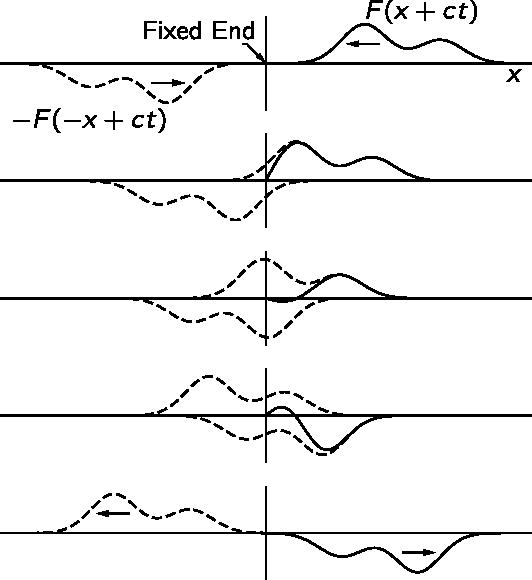
\includegraphics[width=0.7\linewidth]{fyz_fig446.pdf}
      \caption{ 
               (\cite[s.~707]{Feynman01})}
      \label{fyz_fig446}
    \end{figure}

    \begin{figure}[ht!] %\ref{fyz_fig447}
      \centering
      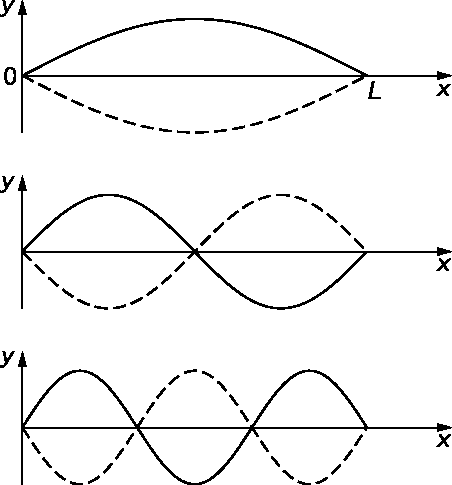
\includegraphics[width=0.7\linewidth]{fyz_fig447.pdf}
      \caption{ 
               (\cite[s.~707]{Feynman01})}
      \label{fyz_fig447}
    \end{figure}

    \begin{figure}[ht!] %\ref{fyz_fig448}
      \centering
      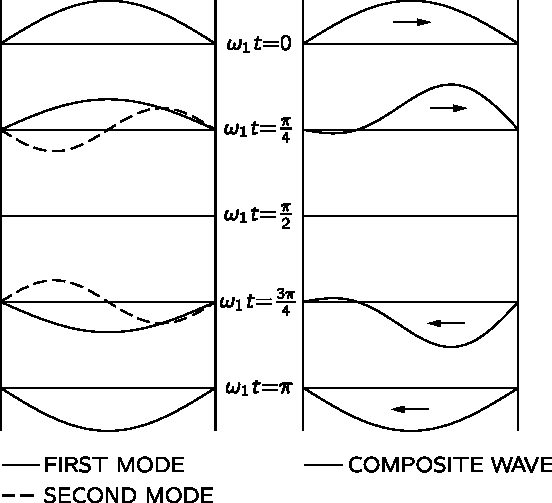
\includegraphics[width=0.7\linewidth]{fyz_fig448.pdf}
      \caption{ 
               (\cite[s.~707]{Feynman01})}
      \label{fyz_fig448}
    \end{figure}

    \begin{figure}[ht!] %\ref{fyz_fig449}
      \centering
      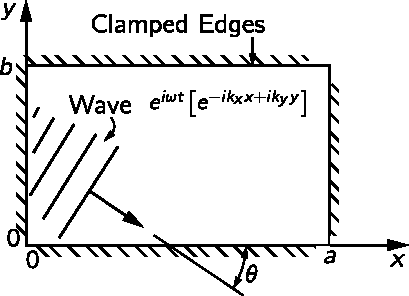
\includegraphics[width=0.7\linewidth]{fyz_fig449.pdf}
      \caption{ 
               (\cite[s.~707]{Feynman01})}
      \label{fyz_fig449}
    \end{figure}

    \begin{figure}[ht!] %\ref{fyz_fig450}
      \centering
      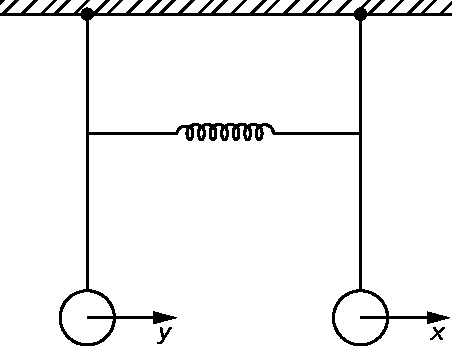
\includegraphics[width=0.7\linewidth]{fyz_fig450.pdf}
      \caption{ 
               (\cite[s.~707]{Feynman01})}
      \label{fyz_fig450}
    \end{figure}